\section{Validación automática de los \glspl{BT}}
\label{sec:Validacion}

Para que los \glspl{BT} generados se considerasen válidos para las pruebas se han tenido en cuenta dos factores: que los árboles generados respeten el órden de los nodos (si hay acciones dependientes unas con otras no deben ejecutarse los hijos antes que los padres) y que deben cumplir un objetivo.
Estas comprobaciones no son obligatorias para el funcionamiento de la herramienta, sino que es un apoyo para automatizar este proceso.

\subsection{Validación de dependencias}
Para comprobar el órden correcto de los nodos se ha recurrido al uso de un autómata finito no determinista, NFA por las siglas en inglés de Non-Deterministic Finite Automata (\cite{NFA}, \cite{NFAPlan}), definido de la siguiente manera:
\begin{itemize}
    \item Los estados son los nodos de \gls{BT}.
    \item Las transiciones son las relaciones padre-hijo.
    \item El alfabeto son las IDs de las tareas.
    \item Hay un conjunto de estados abiertos.
    \item Hay una serie de estados iniciales.
    \item La función de transición es no determinista porque un mismo símbolo puede activar múltiples nodos de forma simultánea, ya que diferentes tareas pueden estar en diferentes puntos del árbol.
\end{itemize}
Este NFA está implementado en la clase ``BehaviorList'', la cual está implementada mediante el patrón Singleton para que todas las tareas puedan acceder a ella.
Para esta verificación se necesita un archivo JSON en el que se especifican las restricciones.
Se puede ver un ejemplo de un JSON con las restricciones en el apéndice \ref{appendix:Orden}.

Una vez se construyan las dependencias mediante el NFA empieza la ejecución del BT.
Para que funcione esta comprobación a la hora de ejecutarse una tarea o un decorador, éste debe llamar a la función ``addBehavior'' de esta clase con el nombre de la tarea.
Cuando llega una tarea nueva se realiza la comprobación de las dependencias de la siguiente forma:

\begin{enumerate}
    \item Se recuperan los nodos candidatos gracias a su ID.
    \item Se crea un nuevo conjunto de nuevos estados.
    \item Si un candidato no tiene padre (no depende de ninguna otra acción) se añade este nodo a los nuevos posibles estados.
    \item Se recorren todos los hijos de los estados activos y se comprueba si coinciden con el ID de la tarea o el decorador actual. En caso afirmativo se añade este hijo al conjunto de nuevos estados.
\end{enumerate}

Al final de la función se comprueba si el conjunto de nuevos estados está vacío.
En el caso de que el conjunto de nuevos estados no está vacío implica que sí se han respetado las dependencias, por lo que éste pasa a ser el conjunto de estados abiertos.
Por el otro lado, si el conjunto de nuevos estados está vacío es que no existe ningún posible estado en el que el órden de la ejecución de los nodos sea la actual, lo que implica que no se han respetado las dependencias y la validación falla.

Para los casos en los que la validación puede fallar se ha creado una clase interfaz ``IValidatorCallback'' que se encarga de gestionar las terminaciones de la validación por fallos o por terminación de la ejecución.
Ya que es la clase ``GeneratorComponent'' quien se encarga de llamar a la herramienta de generación, es esta quien hereda de la interfaz y quien es llamada por la clase ``BehaviorList'' cuando falla la validación, pasándole una lista de todas las acciones ejecutadas hasta el momento y la acción en la que ha fallado.
Es entonces cuando la clase ``GeneratorComponent'' interrumpe el modo de juego y vuelve a llamar a la herramienta con el pseudocódigo fallido, el contexto dado por ``BehaviorList'' y el prompt con la acción original y vuelve a intentar la ejecución cuando la herramienta arregla el psuedocódigo.

\subsection{Validación de objetivos}
Para validar los objetivos específicos de los comportamientos se ha creado una clase interfaz ``ObjectiveValidatorBase'' que contiene un método para comprobar si el objetivo se ha cumplido y un mensaje de error indicando que el objetivo ha fallado.
De esta interfaz deben heredar componentes de Actor para que los objetos ``BTGeneratorManager'' los puedan tener y puedan hacer la comprobación de los objetivos una vez se acabe la ejecución.
Si la comprobación del objetivo es fallida se le pasa a la herramienta el mensaje de error y la lista de tareas ejecutadas, así como el pseudocódigo fallido y el prompt original, y se vuelve a intentar con un pseudocódigo arreglado.

\subsection{Entornos creados para la validación}
Una vez se han tenido los métodos de validación de los BTs se han creado tres entornos con diferentes pruebas.

El primero de ellos consta de tres flores de distintos colores: rojo, azul y amarillo.
En este entorno se le pide a la herramienta que genere un BT donde recoja una única flor de cada tipo, independientemente del órden, con el siguiente prompt: ``NPC that has to choose and pick one flower red, one flower yellow, and one flower blue. In order to pick a flower it has to be first in the position of the flower.''.
Al ser una tarea sencilla la herramienta solo ha necesitado un intento y un tiempo de ejecución de 84.84 segundos para crear un BT válido y que cumpla con el objetivo.

El segundo de los entornos consta de tres flores azules, una flor roja y una flor amarilla, y aquí se le pide a la herramienta que genere un BT que recoja tres flores azules y después una roja mediante el siguiente prompt: ``NPC that has to choose and then pick first three blue flowers, and, after that, has to choose and pick one red flower. In order to pick a flower it has to be first in the position of the flower''.
Al igual que en el caso anterior, solo ha necesitado de un intento y un tiempo de 45.46 segundos para realizar un BT válido.
En la figura \ref{fig:escenario2} se puede ver una captura de pantalla de este entorno.

\begin{figure}[H]
    \centering
    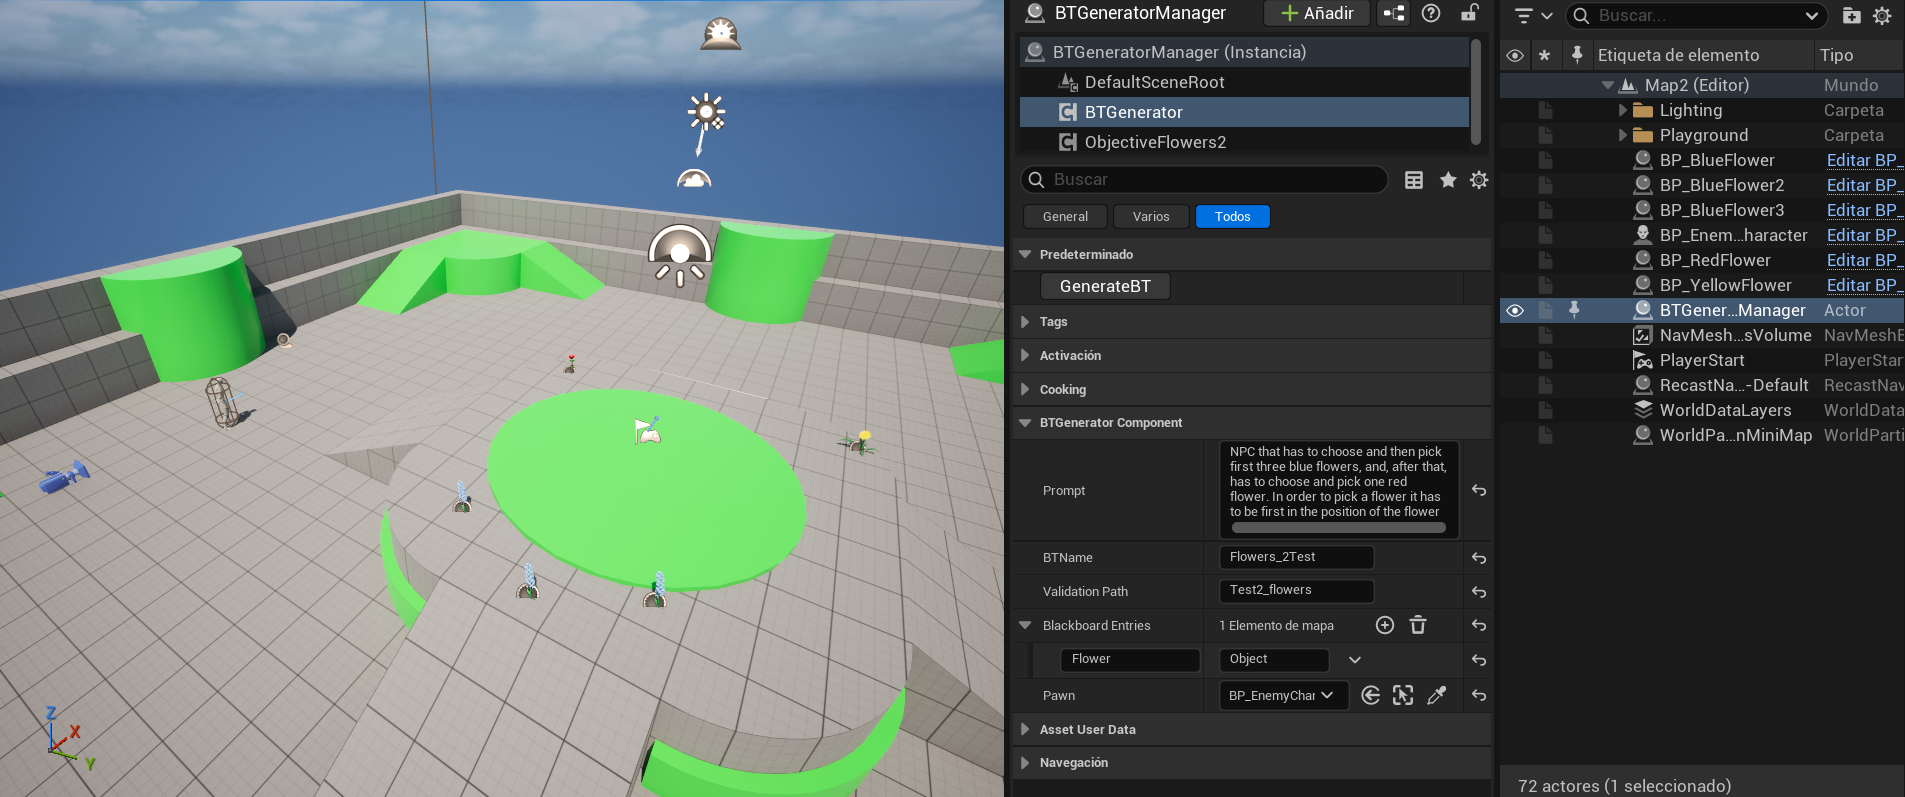
\includegraphics[width=1\textwidth]{Imagenes/Bitmap/Entorno2.png}
    \caption[Captura de pantalla del segundo entorno]{Captura de pantalla del segundo entorno de pruebas de validación.}
    \label{fig:escenario2}
\end{figure}

El tercer entorno consta de un enemigo y un punto de patrulla.
Aquí se le pide a la herramienta que genere un comportamiento clásico en videojuegos: un NPC que patruye el escenario por distintos puntos y, que si ve al jugador, le persiga para atacarle.
Para ello se ha usado el siguiente prompt: ``NPC that has to do one of this two options:
- If the objective is at his line of sight it has to: 1. chase him 2. move to his position 3. if is near the objective, it has to attack him.
- Otherwise, it has to: 1. select a waypoint 2. move to the waypoint''.

A pesar de ser una petición más compleja debido a la naturaleza del comportamiento y al aumento de número de variables de la Blackboard (cuatro variables, dos condicionales para ver si el objetivo está en el punto de mira y si el objetivo está cerca, el punto de patrulla a elegir y el objetivo a perseguir), la herramienta ha sido capaz de generar en 153.1 segundos un BT válido a la primera en cuanto a cumplimiento de objetivos y respetando las dependencias, aunque sí se ha tenido que modificar alguna tarea que requería de una variable de la Blackboard que el segundo LLM no le ha adjudicado ninguna variable.
En la figura \ref{fig:escenario3} se puede ver una captura de pantalla de este tercer entorno.

\begin{figure}[H]
    \centering
    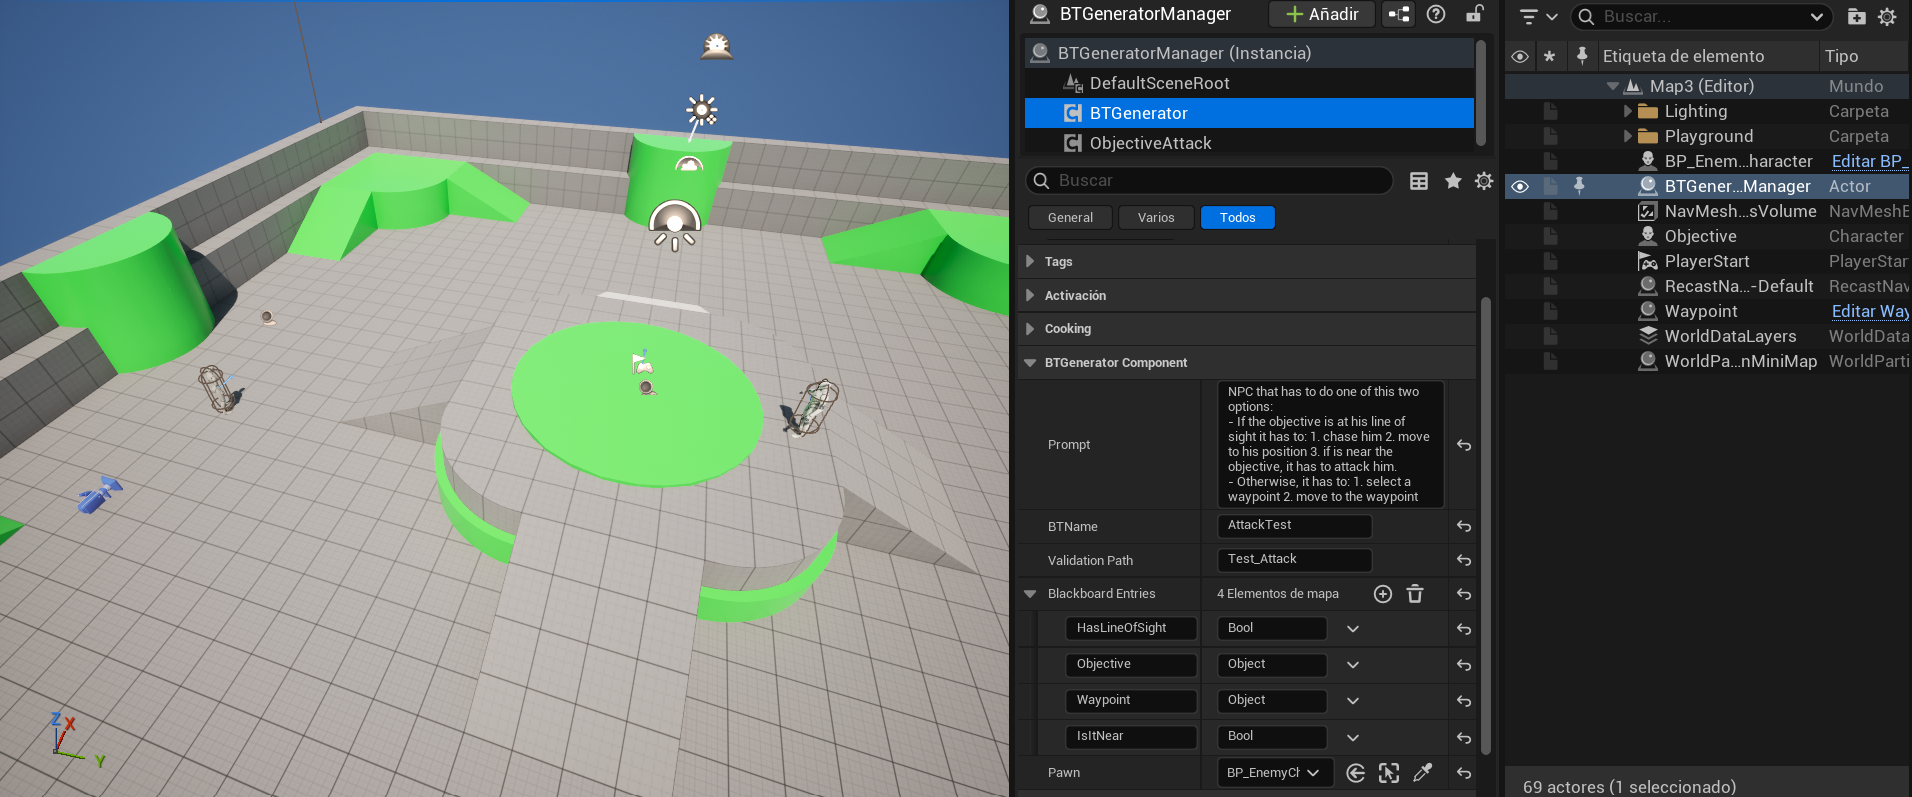
\includegraphics[width=1\textwidth]{Imagenes/Bitmap/Entorno3.png}
    \caption[Captura de pantalla del tercer entorno]{Captura de pantalla del tercer entorno de pruebas de validación.}
    \label{fig:escenario3}
\end{figure}

Con los resultados de esta validación, resumidos en la tabla \ref{tab:validacion}, se ha podido establecer un baseline del funcionamiento de la herramienta para, finalmente, realizar pruebas con usuarios.

\begin{longtblr}[
    caption = {Resultados de las pruebas de validación},
    label = {tab:validacion}
]{
colspec={|l|l|l|},
rowhead=1,
hlines,
row{even}={gray9},
cells   = {font=\footnotesize\linespread{0.84}\selectfont},
}
    \hline
    Entorno    & Intentos  & Tiempo de ejecución\\ \hline
    1    & 1   & 84.84 segundos \\
    2    & 1  & 45.46 segundos \\
    3  & 1  &  153.1 segundos \\ \hline
\end{longtblr}
